% Key Diagrams using TikZ

% Diagram 1: Dual-Track Model
\begin{figure}[htbp]
\centering
\begin{tikzpicture}[
    node distance=1.5cm,
    box/.style={rectangle, draw, minimum width=2.5cm, minimum height=1cm, align=center},
    static/.style={box, fill=blue!20},
    dynamic/.style={box, fill=green!20},
    arrow/.style={->, thick}
]
    % Static Track
    \node[static] (fund) {Fund UTXO\\(Static Anchor)};
    \node[below=0.3cm of fund, align=center] (fund-content) {\small Capacity: $V$\\Participants: $K_p$\\AggVK};
    
    % Dynamic Track
    \node[dynamic, right=4cm of fund] (state) {State UTXO\\(Dynamic Pointer)};
    \node[below=0.3cm of state, align=center] (state-content) {\small Sequence: $n$\\Balances: $R_b$\\PTLCs: $R_p$};
    
    % RefOp operator
    \draw[arrow, dashed, blue, thick] (state) -- node[above] {$\RefOp$ (read-only)} (fund);
    
    % Labels
    \node[above=0.5cm of fund, font=\bfseries] {Static Track};
    \node[above=0.5cm of state, font=\bfseries] {Dynamic Track};
    
\end{tikzpicture}
\caption{Dual-Track State Machine Architecture}
\label{fig:dual-track}
\end{figure}

% Diagram 2: State Transition
\begin{figure}[htbp]
\centering
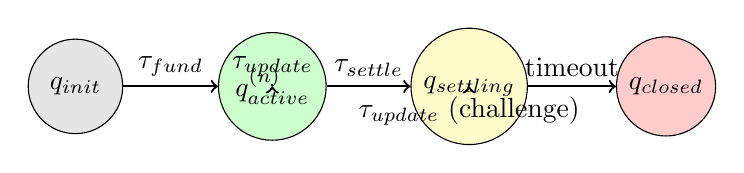
\begin{tikzpicture}[
    node distance=2.5cm,
    state/.style={circle, draw, minimum size=1.2cm, align=center},
    arrow/.style={->, thick}
]
    \node[state, fill=gray!20] (init) {$q_{init}$};
    \node[state, fill=green!20, right of=init] (active) {$q_{active}^{(n)}$};
    \node[state, fill=yellow!20, right of=active] (settling) {$q_{settling}$};
    \node[state, fill=red!20, right of=settling] (closed) {$q_{closed}$};
    
    \draw[arrow] (init) -- node[above] {$\tau_{fund}$} (active);
    \draw[arrow, bend left=30] (active) to node[above] {$\tau_{update}$} (active);
    \draw[arrow] (active) -- node[above] {$\tau_{settle}$} (settling);
    \draw[arrow] (settling) -- node[above] {timeout} (closed);
    \draw[arrow, bend right=40] (settling) to node[below] {$\tau_{update}$ (challenge)} (settling);
    
\end{tikzpicture}
\caption{Channel State Machine Transitions}
\label{fig:state-machine}
\end{figure}

% Diagram 3: Recursive Channel Factory
\begin{figure}[htbp]
\centering
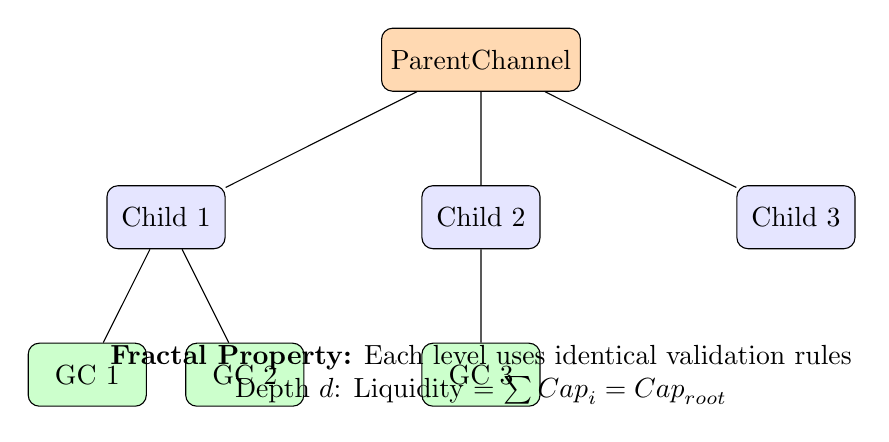
\begin{tikzpicture}[
    level distance=2cm,
    level 1/.style={sibling distance=4cm},
    level 2/.style={sibling distance=2cm},
    channel/.style={rectangle, draw, rounded corners, minimum width=1.5cm, minimum height=0.8cm, fill=blue!10},
    arrow/.style={->, thick}
]
    \node[channel, fill=orange!30] {Parent\\Channel}
        child {node[channel] {Child 1}
            child {node[channel, fill=green!20] {GC 1}}
            child {node[channel, fill=green!20] {GC 2}}
        }
        child {node[channel] {Child 2}
            child {node[channel, fill=green!20] {GC 3}}
        }
        child {node[channel] {Child 3}};
    
    \node[below=3.5cm, align=center] {
        \textbf{Fractal Property:} Each level uses identical validation rules\\
        Depth $d$: Liquidity = $\sum \text{Cap}_i = \text{Cap}_{root}$
    };
\end{tikzpicture}
\caption{Recursive Channel Factory Structure}
\label{fig:recursive-factory}
\end{figure}

% Diagram 4: PTLC Multi-hop Payment
\begin{figure}[htbp]
\centering
\begin{tikzpicture}[
    node distance=3cm,
    party/.style={circle, draw, minimum size=1cm, fill=blue!10},
    arrow/.style={->, thick}
]
    \node[party] (alice) {Alice};
    \node[party, right of=alice] (bob) {Bob};
    \node[party, right of=bob] (carol) {Carol};
    \node[party, right of=carol] (dave) {Dave};
    
    \draw[arrow, blue] (alice) -- node[above, align=center] {PTLC($Q$)} (bob);
    \draw[arrow, blue] (bob) -- node[above, align=center] {PTLC($Q$)} (carol);
    \draw[arrow, blue] (carol) -- node[above, align=center] {PTLC($Q$)} (dave);
    
    \draw[arrow, red, dashed, bend right=50] (dave) to node[below, align=center] {reveal $s$\\(scalar)} (alice);
    
    \node[below=1.5cm of bob, align=center] {
        Once Dave reveals $s$, all hops unlock atomically\\
        $Q = s \cdot G$ (same point lock for all)
    };
\end{tikzpicture}
\caption{PTLC Multi-Hop Atomic Payment}
\label{fig:ptlc-payment}
\end{figure}

% Diagram 5: STPC Mempool Management
\begin{figure}[htbp]
\centering
\begin{tikzpicture}[
    node distance=2cm,
    box/.style={rectangle, draw, minimum width=2cm, minimum height=1cm},
    arrow/.style={->, thick}
]
    % Mempool
    \node[box, fill=gray!20, minimum width=6cm, minimum height=3cm] (mempool) {};
    \node[above=0cm of mempool.north, font=\bfseries] {Mempool};
    
    \node[box, fill=green!20] at (mempool.center) (tip) {State$_{n}$\\(Current Tip)};
    
    % Incoming transactions
    \node[box, fill=blue!10, left=3cm of mempool] (new1) {State$_{n+1}$};
    \node[box, fill=blue!10, above=0.5cm of new1] (new2) {State$_{n}$\\Higher Fee};
    \node[box, fill=red!10, below=0.5cm of new1] (old) {State$_{n-1}$};
    
    % Arrows
    \draw[arrow, green!70!black] (new1) -- node[above] {Replace} (tip);
    \draw[arrow, green!70!black] (new2) -- node[above, sloped] {Replace} (tip);
    \draw[arrow, red] (old) -- node[below] {Reject} (mempool.west |- old);
    
    \node[below=0.5cm of mempool, align=center, font=\small] {
        STPC Rule: Only one state per channel in mempool\\
        Higher sequence or higher fee replaces current tip
    };
\end{tikzpicture}
\caption{STPC (Single-Tip-Per-Channel) Strategy}
\label{fig:stpc}
\end{figure}

% Diagram 6: Transaction Type Enumeration
\begin{figure}[htbp]
\centering
\begin{tikzpicture}[
    node distance=1.2cm,
    box/.style={rectangle, draw, rounded corners, minimum width=2.5cm, minimum height=0.8cm, align=center},
    arrow/.style={->, thick}
]
    \node[box, fill=orange!20] (fund) {FUND\\Create channel};
    \node[box, fill=blue!20, right=2.5cm of fund] (update) {UPDATE\\State iteration};
    \node[box, fill=green!20, right=2.5cm of update] (settle) {SETTLE\\Settlement};
    \node[box, fill=purple!20, right=2.5cm of settle] (splice) {SPLICE\\Topology\\transform};
    
    \node[above=1.5cm of update, box, fill=gray!10, minimum width=10cm] (validator) {
        EltooBlockValidator\\
        $\bigO(1)$ Pattern Matching
    };
    
    \draw[arrow] (validator) -- (fund);
    \draw[arrow] (validator) -- (update);
    \draw[arrow] (validator) -- (settle);
    \draw[arrow] (validator) -- (splice);
    
\end{tikzpicture}
\caption{Transaction Type Enumeration System}
\label{fig:tx-types}
\end{figure}

% Diagram 7: Topology Reconfiguration
\begin{figure}[htbp]
\centering
\begin{tikzpicture}[
    node distance=1.5cm,
    party/.style={circle, draw, minimum size=0.8cm, fill=blue!10},
    channel/.style={draw, thick}
]
    % Before: Ring topology
    \begin{scope}[local bounding box=before]
        \node[party] (a1) {A};
        \node[party, right=1.5cm of a1] (b1) {B};
        \node[party, below=1.5cm of b1] (c1) {C};
        \node[party, left=1.5cm of c1] (d1) {D};
        
        \draw[channel] (a1) -- (b1);
        \draw[channel] (b1) -- (c1);
        \draw[channel] (c1) -- (d1);
        \draw[channel] (d1) -- (a1);
        
        \node[above=0.3cm of a1, font=\bfseries] {Before: Ring};
    \end{scope}
    
    % Arrow
    \node[right=2cm of before.east, font=\Large] {$\xrightarrow{\tau_{splice}}$};
    
    % After: Star topology
    \begin{scope}[local bounding box=after, xshift=8cm]
        \node[party, fill=orange!30] (hub) {Hub};
        \node[party, above left=1cm of hub] (a2) {A};
        \node[party, above right=1cm of hub] (b2) {B};
        \node[party, below right=1cm of hub] (c2) {C};
        \node[party, below left=1cm of hub] (d2) {D};
        
        \draw[channel] (hub) -- (a2);
        \draw[channel] (hub) -- (b2);
        \draw[channel] (hub) -- (c2);
        \draw[channel] (hub) -- (d2);
        
        \node[above=0.5cm of hub, font=\bfseries] {After: Star};
    \end{scope}
    
    \node[below=2cm of before.south, align=center] {
        \textbf{Atomic Reconfiguration:} Single $\tau_{splice}$ transaction\\
        transforms entire topology while preserving total value
    };
\end{tikzpicture}
\caption{Topology Reconfiguration: Ring to Star}
\label{fig:topology-reconfig}
\end{figure}
